% ============================================================
% CHAPTER 3: STUDY AREA AND DATA
% ============================================================
\chapter{Study Area and Data}
\label{ch:data}

\section{Study Area: The West Midlands}
\label{sec:study-area}

The study focuses on the West Midlands metropolitan region. Located in central England, it comprises the seven metropolitan boroughs of Birmingham, Coventry, Dudley, Sandwell, Solihull, Walsall, and Wolverhampton. With a population of over 3 million \parencite{officefornationalstatistics2025}, the West Midlands is the second largest and second most populated conurbation in Britain after London \parencite{westmidlandscombinedauthority2025}. As Figure~\ref{fig:study-area} illustrates, the region exhibits a polycentric urban structure, with Birmingham as the dominant core surrounded by smaller but densely populated centres including Wolverhampton, Coventry, and the towns of the Black Country \footnote{The Black Country refers to the area immediately west and northwest of Birmingham, comprising the metropolitan boroughs of Dudley, Sandwell, Walsall, and Wolverhampton.}, While the southern and eastern portions of Solihull and the fringes of Walsall and Birmingham are predominantly rural. This mix of dense urban centres and lower-density peripheral areas presents distinct challenges for cycling infrastructure provision, as routes must negotiate fragmented land uses, varying traffic conditions, and considerable trip distances between centres \parencite{delclos-alio2024}.

\begin{figure}[h]
  \centering
  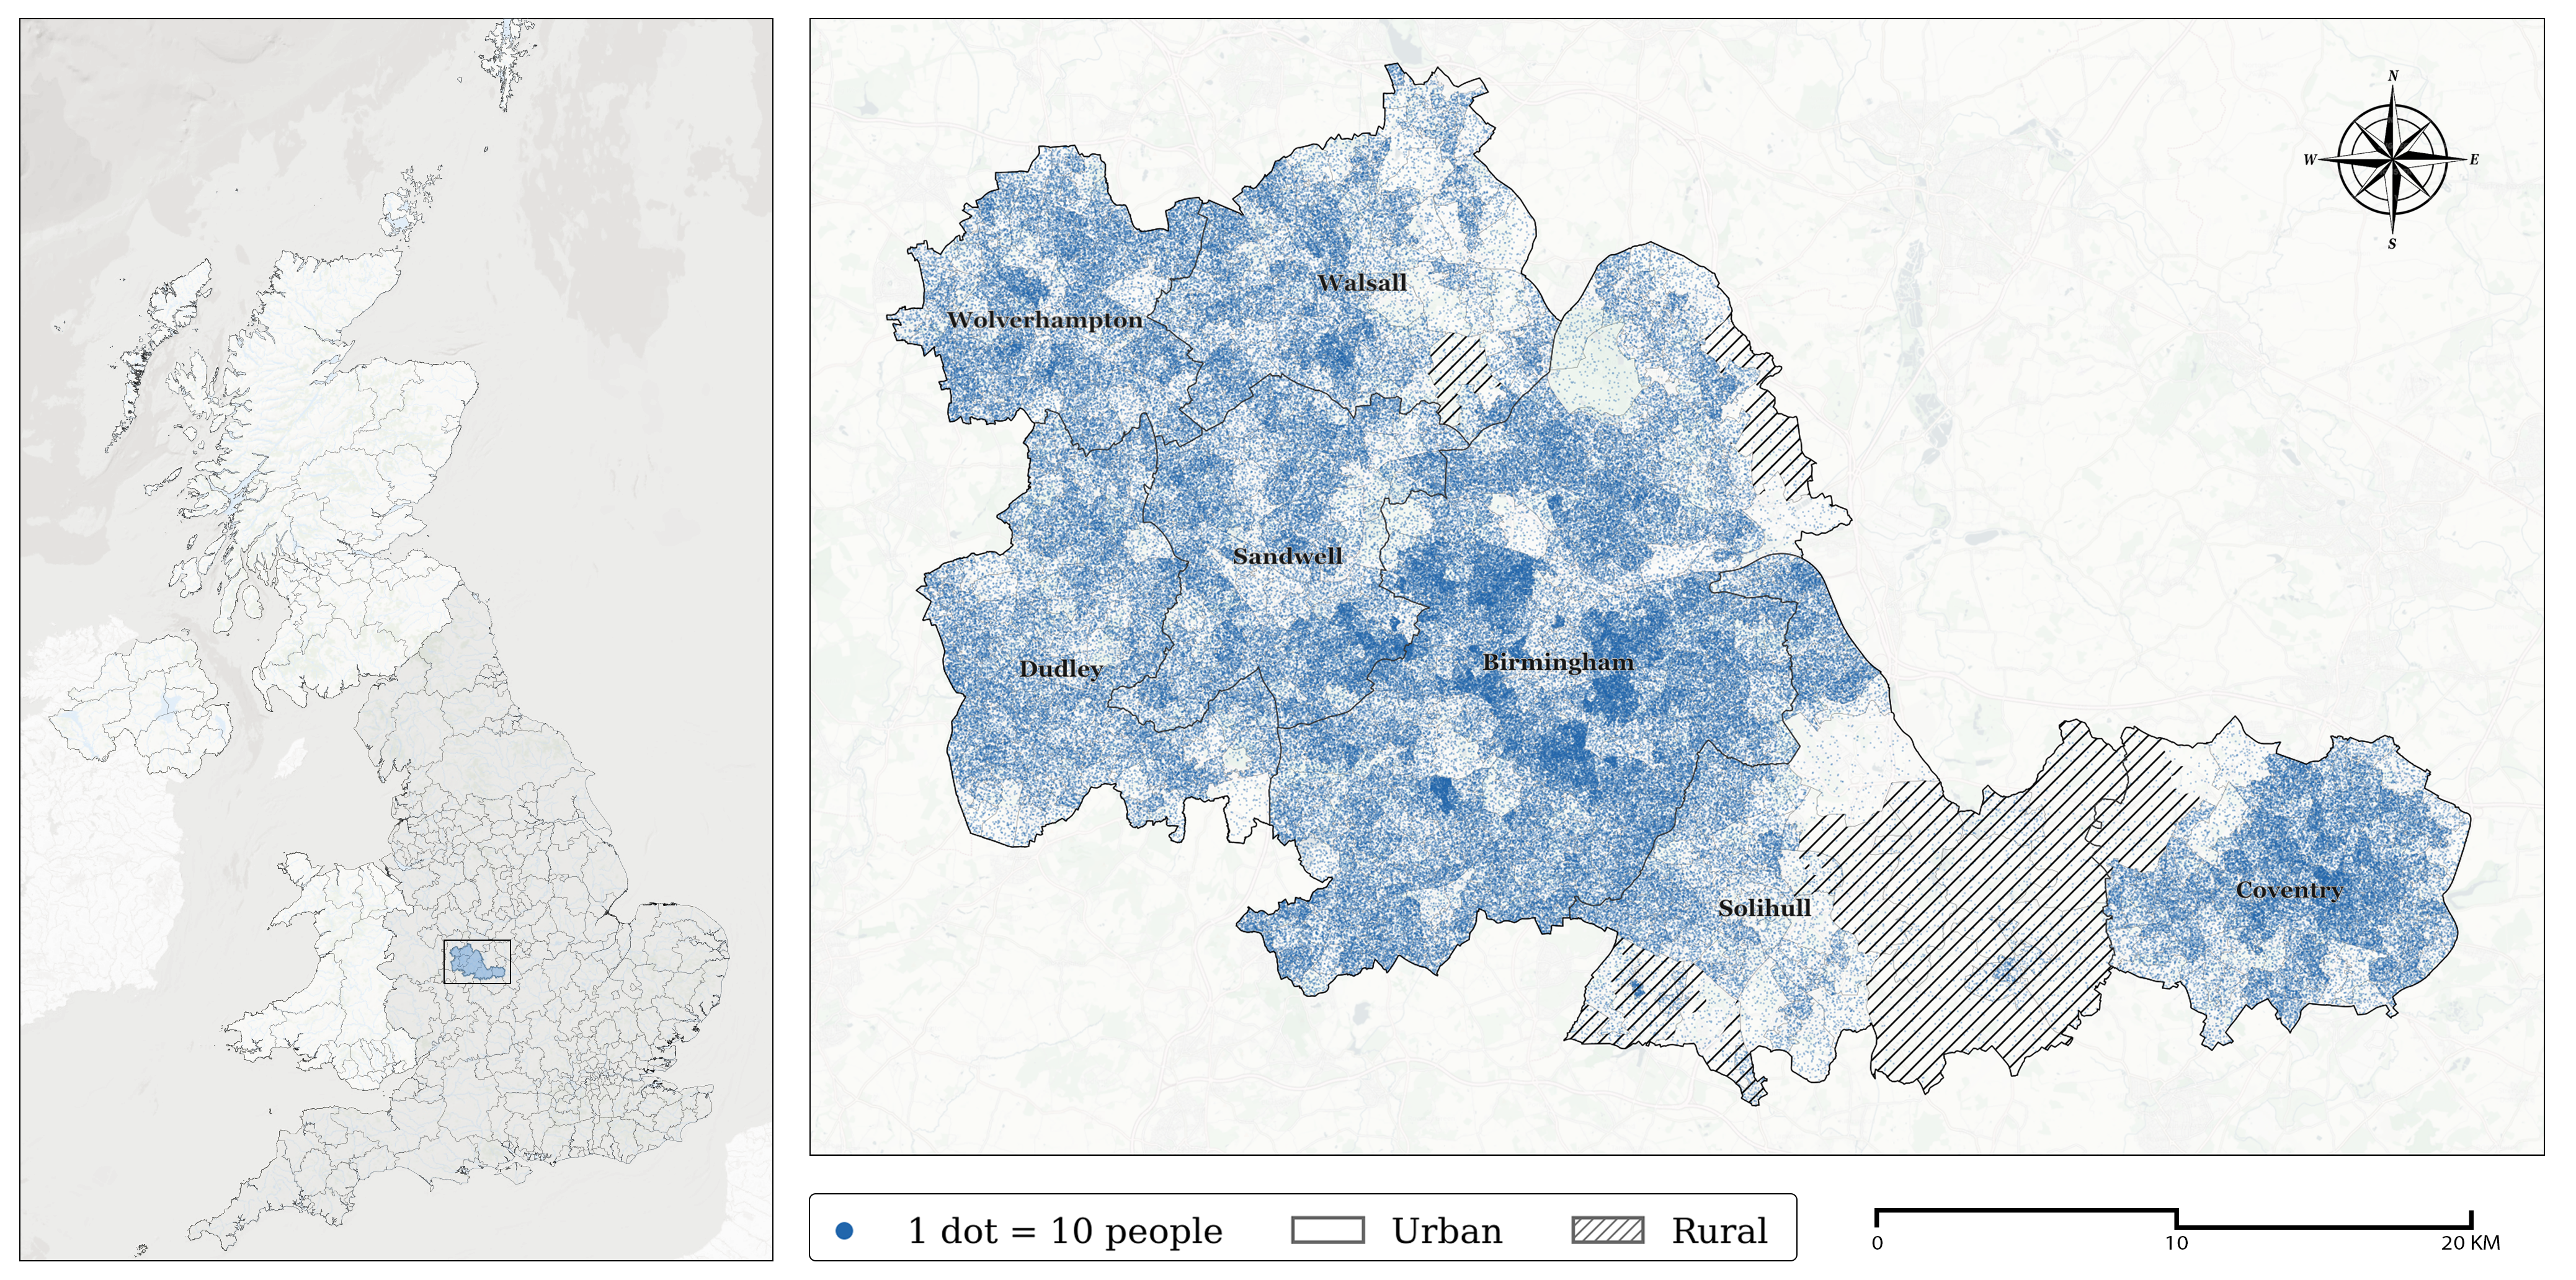
\includegraphics[width=\textwidth]{Figure/study_area_map.png}
  \caption[Study area: The West Midlands]{Study Area: The West Midlands.}
  \label{fig:study-area}
\end{figure}
 
The West Midlands has been a centre of British automobile manufacturing since the early twentieth century, accounting for approximately 60\% of national car production in the early 1970s \parencite{donnelly2017}. Its urban fabric bears this legacy: post-war interventions such as Birmingham's Inner Ring Road, completed in 1971 as Britain's first urban motorway \parencite{gunn2018}, entrenched car-oriented mobility across the region, exemplifying what \textcite{mattioli2020} characterise as a self-reinforcing car-dependent system. National Travel Survey data show that the wider West Midlands region \footnote{The wider West Midlands region includes the seven metropolitan boroughs as well as the surrounding counties of Herefordshire, Shropshire, Staffordshire, Warwickshire, and Worcestershire.} consistently records the highest share of private motorised trips among English regions, at 69\% in 2024 \parencite{departmentfortransport2025}. And cycling accounts for only approximately 0.9\% of all trips in the metropolitan area \parencite{westmidlandscombinedauthority2024}, despite 41\% of car journeys being under two miles \parencite{westmidlandscombinedauthority2019}. 

In response, Transport for West Midlands (TfWM) has set out an ambitious active travel agenda centred on the Starley Network, a planned 500-mile network of traffic-free or physically separated cycle routes \parencite{westmidlandscombinedauthority2020}, aligned with the national Gear Change vision and LTN 1/20 design standards. Yet the gap between this policy ambition and the region's measurable network-level cycling conditions remains poorly quantified, making the West Midlands a compelling case for the standards-based infrastructure assessment developed in this study.

\section{Data Sources: Overview}
\label{sec:data}

The analytical pipeline draws on four principal data sources. The primary source is Ordnance Survey National Geographic Database Transport (OS NGD Transport), which provides network geometry, road classification, carriageway and cycle lane width, legal access designation, junction type and probe-vehicle-derived average speeds for constructing the directed, stress-classified network (Sections~\ref{sec:method-extraction}--\ref{sec:method-junctionlts}). The Cycle Lane feature collection, achieving full national coverage in March 2026 \parencite{ordnancesurvey2026e}, makes this study one of the first to incorporate authoritative national cycling infrastructure data into a network-level assessment. Department for Transport road traffic count data supply observed AADT volumes and training observations for minor road volume estimation (Section~\ref{sec:method-linklts}). OpenStreetMap (OSM) contributes cycling geometries for Path Link cross-validation, traffic signal locations for junction classification, and school locations for accessibility analysis (Sections~\ref{sec:method-extraction}, \ref{sec:method-junctionlts}, \ref{sec:method-analysis}). Census data from the Office for National Statistics provide MSOA-level commuting flows for OD connectivity and network growth evaluations, and LSOA-level population and boundaries for density and reach analyses (Sections~\ref{sec:method-analysis}--\ref{sec:method-growth}). Table~\ref{tab:datasets} summarises each dataset.

\begin{table}[H]
  \centering
  \caption{Datasets used in this study.}
  \label{tab:datasets}
  \small
  \begin{tabularx}{\textwidth}{l l X l l}
    \toprule
    \textbf{Dataset} & \textbf{Provider} & \textbf{Key Variables} & \textbf{Spatial Unit}  \\
    \midrule
    Road Links        & OS NGD & Geometry, classification, description, width & Edge \\
    Path Links        & OS NGD & Geometry, cycle lane presence & Edge  \\
    Highway Dedication & OS NGD & Legal access designation & Edge  \\
    Cycle Lane        & OS NGD & Facility type, width, placement side & Edge  \\
    Average Speed (RAMI) & OS NGD & Probe-derived average speed & Edge  \\
    Road Node         & OS NGD & Node form, geometry, description & Node  \\
    Path Node         & OS NGD & Node geometry & Node  \\
    \midrule
    Road Traffic Counts & DfT  & AADT by vehicle type & Count point  \\
    \midrule
    Cycling Network   & OSM   & Highway and cycleway tags & Way  \\
    Traffic Signals   & OSM   & Signal node locations & Node  \\
    Schools           & OSM   & Location & Point  \\
    \midrule
    Commuting Flows   & ONS   & OD pairs within 8\,km & MSOA  \\
    Population        & ONS   & Resident population & LSOA \\
    Boundaries        & ONS   & LSOA/MSOA polygons & Polygon \\
    \bottomrule
  \end{tabularx}
\end{table}

\section{Statement of Ethics}
\label{sec:ethics}

This dissertation received ethical approval from the UCL Research Ethics Committee (reference: 3797). Ordnance Survey National Geographic Database data, licensed under the Public Sector Geospatial Agreement and not openly available, were provided by Transport for West Midlands under a formal data transfer agreement; all restricted datasets were stored on UCL-managed OneDrive. Semi-structured interviews with five transport practitioners were conducted with informed consent, and responses were fully anonymised in all outputs. No other personal or individually identifiable data were collected or processed.